% Options for packages loaded elsewhere
% Options for packages loaded elsewhere
\PassOptionsToPackage{unicode}{hyperref}
\PassOptionsToPackage{hyphens}{url}
%
\documentclass[
  oneside,
  open=any,
  fontsize=11pt]{scrbook}
\usepackage{xcolor}
\usepackage{amsmath,amssymb}
\setcounter{secnumdepth}{5}
\usepackage{iftex}
\ifPDFTeX
  \usepackage[T1]{fontenc}
  \usepackage[utf8]{inputenc}
  \usepackage{textcomp} % provide euro and other symbols
\else % if luatex or xetex
  \usepackage{unicode-math} % this also loads fontspec
  \defaultfontfeatures{Scale=MatchLowercase}
  \defaultfontfeatures[\rmfamily]{Ligatures=TeX,Scale=1}
\fi
\usepackage{lmodern}
\ifPDFTeX\else
  % xetex/luatex font selection
\fi
% Use upquote if available, for straight quotes in verbatim environments
\IfFileExists{upquote.sty}{\usepackage{upquote}}{}
\IfFileExists{microtype.sty}{% use microtype if available
  \usepackage[]{microtype}
  \UseMicrotypeSet[protrusion]{basicmath} % disable protrusion for tt fonts
}{}
\makeatletter
\@ifundefined{KOMAClassName}{% if non-KOMA class
  \IfFileExists{parskip.sty}{%
    \usepackage{parskip}
  }{% else
    \setlength{\parindent}{0pt}
    \setlength{\parskip}{6pt plus 2pt minus 1pt}}
}{% if KOMA class
  \KOMAoptions{parskip=half}}
\makeatother
% Make \paragraph and \subparagraph free-standing
\makeatletter
\ifx\paragraph\undefined\else
  \let\oldparagraph\paragraph
  \renewcommand{\paragraph}{
    \@ifstar
      \xxxParagraphStar
      \xxxParagraphNoStar
  }
  \newcommand{\xxxParagraphStar}[1]{\oldparagraph*{#1}\mbox{}}
  \newcommand{\xxxParagraphNoStar}[1]{\oldparagraph{#1}\mbox{}}
\fi
\ifx\subparagraph\undefined\else
  \let\oldsubparagraph\subparagraph
  \renewcommand{\subparagraph}{
    \@ifstar
      \xxxSubParagraphStar
      \xxxSubParagraphNoStar
  }
  \newcommand{\xxxSubParagraphStar}[1]{\oldsubparagraph*{#1}\mbox{}}
  \newcommand{\xxxSubParagraphNoStar}[1]{\oldsubparagraph{#1}\mbox{}}
\fi
\makeatother


\usepackage{longtable,booktabs,array}
\usepackage{calc} % for calculating minipage widths
% Correct order of tables after \paragraph or \subparagraph
\usepackage{etoolbox}
\makeatletter
\patchcmd\longtable{\par}{\if@noskipsec\mbox{}\fi\par}{}{}
\makeatother
% Allow footnotes in longtable head/foot
\IfFileExists{footnotehyper.sty}{\usepackage{footnotehyper}}{\usepackage{footnote}}
\makesavenoteenv{longtable}
\usepackage{graphicx}
\makeatletter
\newsavebox\pandoc@box
\newcommand*\pandocbounded[1]{% scales image to fit in text height/width
  \sbox\pandoc@box{#1}%
  \Gscale@div\@tempa{\textheight}{\dimexpr\ht\pandoc@box+\dp\pandoc@box\relax}%
  \Gscale@div\@tempb{\linewidth}{\wd\pandoc@box}%
  \ifdim\@tempb\p@<\@tempa\p@\let\@tempa\@tempb\fi% select the smaller of both
  \ifdim\@tempa\p@<\p@\scalebox{\@tempa}{\usebox\pandoc@box}%
  \else\usebox{\pandoc@box}%
  \fi%
}
% Set default figure placement to htbp
\def\fps@figure{htbp}
\makeatother





\setlength{\emergencystretch}{3em} % prevent overfull lines

\providecommand{\tightlist}{%
  \setlength{\itemsep}{0pt}\setlength{\parskip}{0pt}}



 


\makeatletter
\@ifpackageloaded{caption}{}{\usepackage{caption}}
\AtBeginDocument{%
\ifdefined\contentsname
  \renewcommand*\contentsname{Table of contents}
\else
  \newcommand\contentsname{Table of contents}
\fi
\ifdefined\listfigurename
  \renewcommand*\listfigurename{List of Figures}
\else
  \newcommand\listfigurename{List of Figures}
\fi
\ifdefined\listtablename
  \renewcommand*\listtablename{List of Tables}
\else
  \newcommand\listtablename{List of Tables}
\fi
\ifdefined\figurename
  \renewcommand*\figurename{Figure}
\else
  \newcommand\figurename{Figure}
\fi
\ifdefined\tablename
  \renewcommand*\tablename{Table}
\else
  \newcommand\tablename{Table}
\fi
}
\@ifpackageloaded{float}{}{\usepackage{float}}
\floatstyle{ruled}
\@ifundefined{c@chapter}{\newfloat{codelisting}{h}{lop}}{\newfloat{codelisting}{h}{lop}[chapter]}
\floatname{codelisting}{Listing}
\newcommand*\listoflistings{\listof{codelisting}{List of Listings}}
\makeatother
\makeatletter
\makeatother
\makeatletter
\@ifpackageloaded{caption}{}{\usepackage{caption}}
\@ifpackageloaded{subcaption}{}{\usepackage{subcaption}}
\makeatother
\usepackage{bookmark}
\IfFileExists{xurl.sty}{\usepackage{xurl}}{} % add URL line breaks if available
\urlstyle{same}
\hypersetup{
  pdftitle={Strategic Resilience and Financial Performance Profile for Scania Logistics NL},
  pdfauthor={Ronald de Boer},
  hidelinks,
  pdfcreator={LaTeX via pandoc}}


\title{Strategic Resilience and Financial Performance Profile for Scania
Logistics NL}
\usepackage{etoolbox}
\makeatletter
\providecommand{\subtitle}[1]{% add subtitle to \maketitle
  \apptocmd{\@title}{\par {\large #1 \par}}{}{}
}
\makeatother
\subtitle{An In-depth Analysis by the Supply Chain Finance Lectoraat,
Hogeschool Windesheim}
\author{Ronald de Boer}
\date{}
\begin{document}
\frontmatter
\maketitle

\renewcommand*\contentsname{Table of contents}
{
\setcounter{tocdepth}{2}
\tableofcontents
}
\listoffigures
\listoftables

\mainmatter
\newpage

\chapter{Executive Summary}\label{executive-summary}

This Strategic Resilience and Financial Performance Profile, prepared by
the Supply Chain Finance Lectoraat at Hogeschool Windesheim, provides
\textbf{Scania Logistics NL} with a rigorous, data-driven analysis of
its supply chain resilience. In an increasingly interconnected and
unpredictable global economy, the capacity to anticipate, withstand, and
adapt to disruptions is not merely an operational advantage but a
critical determinant of financial stability and long-term market
leadership for logistics providers. This report translates resilience
metrics into actionable strategic insights, enabling \textbf{Scania
Logistics NL} to make informed decisions.

\textbf{Overall Supply Chain Resilience Score (SCRES) for Scania
Logistics NL:} \textbf{2.96 / 5.00}

This SCRES provides a holistic benchmark of \textbf{Scania Logistics
NL}'s current capabilities to anticipate, absorb, adapt, and recover
from supply chain disruptions.

\textbf{Key Strategic Insights:}

\begin{itemize}
\tightlist
\item
  \textbf{Operational Strengths:} The assessment identifies core
  strengths within \textbf{Scania Logistics NL}'s logistics operations
  that currently bolster its resilience. These are valuable assets that
  can be leveraged to enhance service reliability and build client
  confidence. \emph{(Specific high-scoring areas will be detailed in the
  main report based on Scania Logistics NL's unique profile).}
\item
  \textbf{Opportunities for Strategic Enhancement:} The analysis also
  highlights specific areas where targeted investments and process
  improvements can yield substantial gains in resilience. Addressing
  these proactively can mitigate potential financial and operational
  impacts of future disruptions. \emph{(Specific areas for improvement
  will be detailed based on Scania Logistics NL's unique profile).}
\item
  \textbf{Financial Resilience Linkages:} Throughout this report,
  emphasis is placed on the critical interplay between operational
  resilience and financial health. A resilient supply chain directly
  contributes to more predictable cash flows, optimized working capital,
  and a stronger financial position, which is increasingly scrutinized
  by stakeholders and financial institutions.
\end{itemize}

\textbf{Path Forward:}

This profile serves as a foundational tool for strategic dialogue within
\textbf{Scania Logistics NL}. We recommend utilizing these insights to
prioritize initiatives that not only strengthen operational resilience
but also enhance long-term financial robustness and market leadership.
The Supply Chain Finance Lectoraat is prepared to support \textbf{Scania
Logistics NL} in translating these findings into impactful strategies.

\newpage

\chapter{Introduction: The Imperative of Resilience in Modern
Logistics}\label{introduction-the-imperative-of-resilience-in-modern-logistics}

The contemporary logistics landscape is characterized by unprecedented
volatility, driven by geopolitical shifts, climate-related disruptions,
technological advancements, and dynamic market demands. For logistic
providers like \textbf{Scania Logistics NL}, the ability to maintain
operational continuity and deliver consistently under such pressures is
no longer a competitive edge but a fundamental requirement for survival
and growth. This is the essence of supply chain resilience.

This report, produced by the Supply Chain Finance Lectoraat at
Hogeschool Windesheim through its Resilience Scan initiative (in
collaboration with NEXT GEN Logistics), provides \textbf{Scania
Logistics NL} with an in-depth assessment of its current supply chain
resilience. Our approach integrates operational analysis with an
understanding of the profound financial implications of resilience. A
resilient supply chain is not merely about mitigating disruptions; it is
intrinsically linked to financial health---affecting working capital,
risk exposure, cost structures, and ultimately, shareholder value.

The Resilience Scan evaluates \textbf{Scania Logistics NL}'s
capabilities across three critical pillars of its operations (Upstream,
Internal, Downstream) and five core dimensions: * \textbf{Resilience
(R):} The innate ability to withstand shocks and recover effectively. *
\textbf{Connectivity (C):} The quality of information sharing and
collaboration across the network. * \textbf{Financial (F):} The fiscal
strength to absorb impacts and fund recovery. * \textbf{Visibility (V):}
The clarity of insight into end-to-end operations. * \textbf{Agility
(A):} The speed and effectiveness of response to change.

The overall Supply Chain Resilience Score (SCRES) for \textbf{Scania
Logistics NL} is \textbf{2.96} (on a 0-5 scale). This report dissects
this score, offering a clear view of current capabilities and a robust
foundation for strategic enhancements aimed at building a more secure
and prosperous future for \textbf{Scania Logistics NL}.

\chapter{Overall Resilience Profile: A Strategic View of Scania
Logistics NL's
Operations}\label{overall-resilience-profile-a-strategic-view-of-scania-logistics-nls-operations}

This section provides a strategic overview of \textbf{Scania Logistics
NL}'s resilience across the three core pillars of its supply chain:
Upstream, Internal Operations, and Downstream. These pillars represent
distinct but interconnected stages where resilience capabilities are
paramount. The scores reflect an aggregation of the five underlying
dimensions, offering insights into broad areas of operational strength
and potential vulnerability. For a logistic provider, understanding this
pillar-level performance is key to ensuring end-to-end service integrity
and mitigating financial risks associated with disruptions in any
segment.

\begin{figure}[H]

{\centering 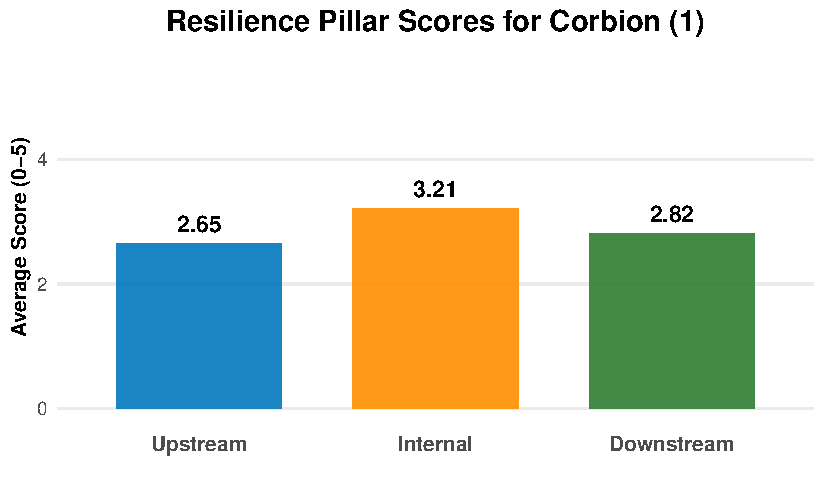
\includegraphics[width=1\linewidth,height=\textheight,keepaspectratio]{example_3_files/figure-pdf/pillar-scores-chart-1.pdf}

}

\caption{Average Resilience Pillar Scores for Scania Logistics NL}

\end{figure}%

The chart above provides a visual synthesis of \textbf{Scania Logistics
NL}'s resilience across its primary operational segments. A balanced
profile often indicates consistent resilience management, yet strategic
priorities may result in differential strengths. For example, a
logistics firm heavily reliant on global sourcing might prioritize
\emph{Upstream} resilience, while one focused on last-mile excellence
might emphasize \emph{Downstream} capabilities. Weaknesses in any pillar
can create bottlenecks, increase costs, and impact service delivery,
ultimately affecting financial performance and client relationships.
This high-level view guides \textbf{Scania Logistics NL} in allocating
resources effectively to fortify its overall resilience posture.

\chapter{Detailed Resilience Dimensions: Unpacking Scania Logistics NL's
Capabilities}\label{detailed-resilience-dimensions-unpacking-scania-logistics-nls-capabilities}

This section delves deeper into the five core dimensions of supply chain
resilience, analyzing \textbf{Scania Logistics NL}'s performance within
each of the Upstream, Internal, and Downstream pillars. Understanding
these granular scores is essential for identifying specific levers for
improvement. Each dimension contributes uniquely to the overall
resilience and has direct implications for a logistic provider's
operational efficiency and financial stability.

\begin{itemize}
\tightlist
\item
  \textbf{Resilience (R):} This dimension reflects the inherent
  robustness and recovery capabilities. Strong R capabilities minimize
  downtime and associated costs, directly impacting profitability and
  potentially reducing insurance liabilities.
\item
  \textbf{Connectivity (C):} Effective C ensures seamless information
  flow and collaboration. For logistic providers, this translates to
  operational efficiencies, reduced errors (cost savings), and stronger
  partner ecosystems, which can be vital for accessing flexible capacity
  or alternative solutions during disruptions.
\item
  \textbf{Financial (F):} This dimension addresses the financial
  capacity to withstand shocks. Adequate F resilience ensures
  \textbf{Scania Logistics NL} can absorb temporary losses, fund
  recovery efforts without jeopardizing core operations, and maintain
  stakeholder confidence, which can influence access to and cost of
  capital.
\item
  \textbf{Visibility (V):} High V provides clear insight into the
  end-to-end supply chain. This enables proactive risk identification,
  optimized inventory (impacting working capital), and efficient
  resource allocation, thereby reducing the financial impact of
  unforeseen events.
\item
  \textbf{Agility (A):} This signifies the ability to respond swiftly
  and adapt effectively. For a logistic provider, A allows for rapid
  rerouting, mode-switching, or service adjustments, minimizing
  disruption costs, retaining customers, and potentially capturing
  opportunities arising from market shifts.
\end{itemize}

\section{Upstream Resilience
Dimensions}\label{upstream-resilience-dimensions}

This analysis focuses on \textbf{Scania Logistics NL}'s resilience
capabilities in its interactions with suppliers and the management of
inbound logistics. Effective upstream resilience is crucial for ensuring
the consistent flow of goods and services that underpin \textbf{Scania
Logistics NL}'s operations.

\begin{figure}[H]

{\centering 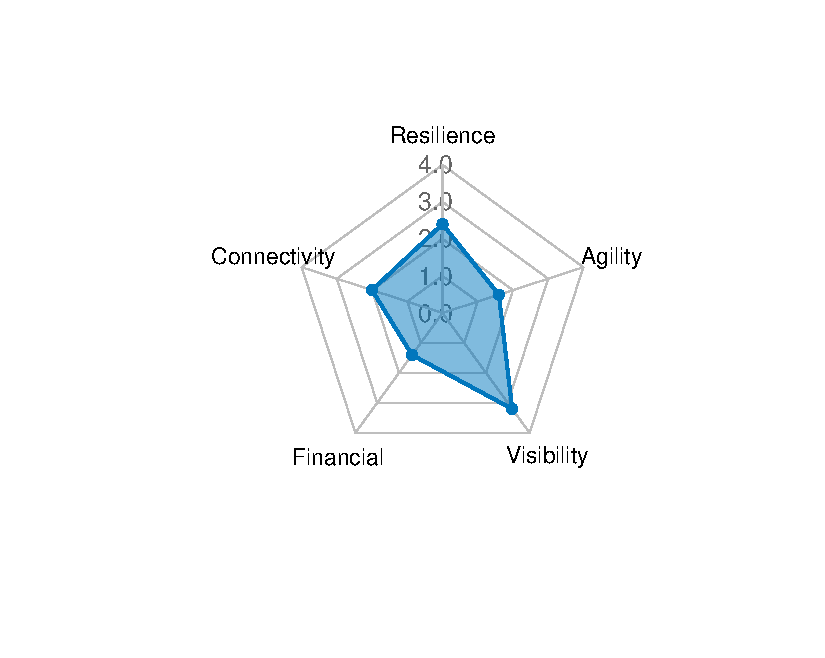
\includegraphics[width=0.8\linewidth,height=\textheight,keepaspectratio]{example_3_files/figure-pdf/upstream-radar-chart-1.pdf}

}

\caption{Upstream Resilience Dimensions for Scania Logistics NL}

\end{figure}%

The profile above reveals \textbf{Scania Logistics NL}'s specific
strengths and vulnerabilities in its upstream operations. For example, a
high score in Upstream \emph{Connectivity} can significantly reduce
information asymmetries with suppliers, leading to better planning and
reduced buffer stocks (positively impacting working capital).
Conversely, a low score in Upstream \emph{Financial} (e.g., assessing
supplier financial health) could expose \textbf{Scania Logistics NL} to
significant disruption if key suppliers face financial distress.

\section{Internal Operational Resilience
Dimensions}\label{internal-operational-resilience-dimensions}

This section scrutinizes the resilience embedded within \textbf{Scania
Logistics NL}'s core internal operations, including warehousing, fleet
management, technological infrastructure, and human capital. The
robustness of these internal processes is fundamental to consistent
service delivery and cost control.

\begin{figure}[H]

{\centering 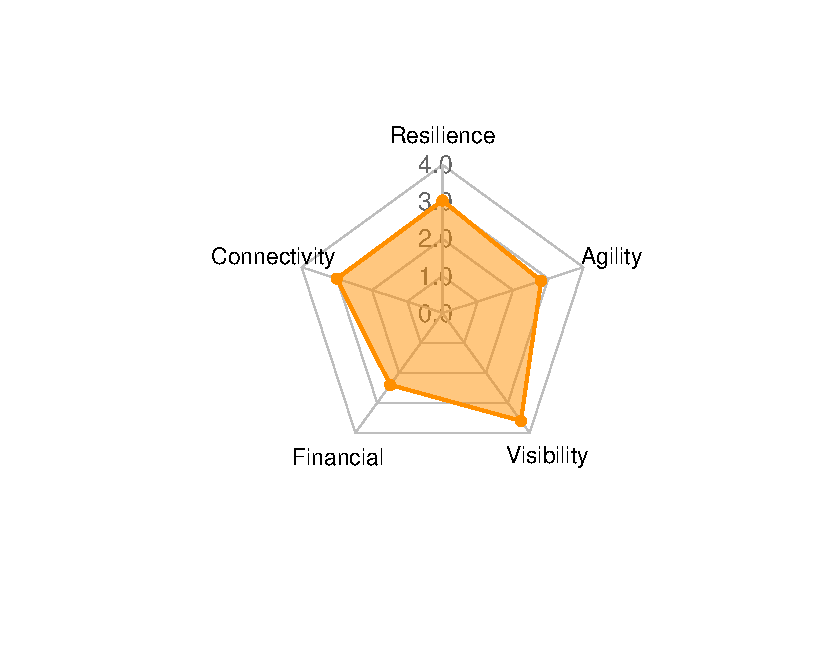
\includegraphics[width=0.8\linewidth,height=\textheight,keepaspectratio]{example_3_files/figure-pdf/internal-radar-chart-1.pdf}

}

\caption{Internal Operational Resilience Dimensions for Scania Logistics
NL}

\end{figure}%

Within \textbf{Scania Logistics NL}'s internal operations, strong
\emph{Agility} allows for rapid adaptation to demand shifts or resource
constraints, minimizing overtime costs and service penalties. High
\emph{Visibility} into internal processes (e.g., asset utilization,
warehouse capacity) enables optimized resource deployment and proactive
maintenance, reducing the likelihood of costly operational failures. The
\emph{Financial} dimension here reflects the capacity to absorb costs
from internal disruptions, such as equipment breakdown or IT system
recovery.

\section{Downstream Resilience
Dimensions}\label{downstream-resilience-dimensions}

This analysis evaluates \textbf{Scania Logistics NL}'s resilience in its
downstream activities, which directly interface with customers and
markets. This includes distribution networks, final-mile delivery, and
customer communication protocols, all critical for maintaining revenue
streams and customer loyalty.

\begin{figure}[H]

{\centering 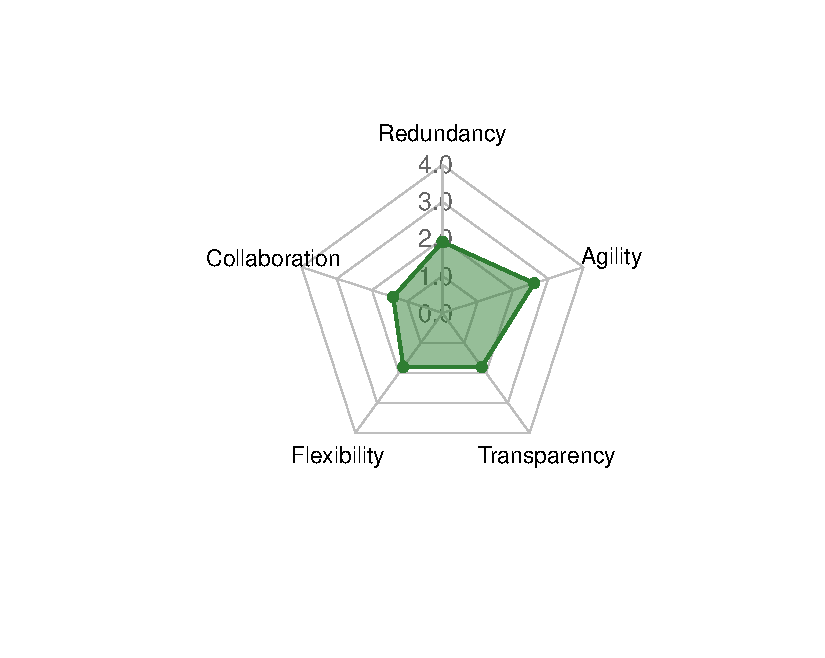
\includegraphics[width=0.8\linewidth,height=\textheight,keepaspectratio]{example_3_files/figure-pdf/downstream-radar-chart-1.pdf}

}

\caption{Downstream Resilience Dimensions for Scania Logistics NL}

\end{figure}%

In the downstream segment, high \emph{Connectivity} with customers
allows \textbf{Scania Logistics NL} to manage expectations effectively
during disruptions, preserving goodwill. Strong \emph{Visibility} into
final-mile operations can identify potential delivery issues
proactively, reducing failed delivery costs and enhancing customer
satisfaction. The \emph{Resilience} dimension here reflects the ability
to quickly restore customer-facing services after an outage,
safeguarding revenue and market reputation.

\chapter{Materials and Methods}\label{materials-and-methods}

The insights presented in this Strategic Resilience Profile for
\textbf{Scania Logistics NL} are derived from data collected via the
Resilience Scan, an evidence-based self-assessment instrument developed
by the Supply Chain Finance Lectoraat at Hogeschool Windesheim. The
Resilience Scan is grounded in extensive research into supply chain risk
management, organizational resilience, and financial performance
indicators.

Participants from \textbf{Scania Logistics NL} completed a structured
questionnaire, providing ratings on their perceived capabilities across
the five core dimensions of resilience (Resilience, Connectivity,
Financial, Visibility, and Agility) within the three operational pillars
(Upstream, Internal, and Downstream). These qualitative perceptions are
systematically converted into quantitative scores (typically on a 1-5
scale), which are then aggregated to produce the dimension, pillar, and
the overall Supply Chain Resilience Score (SCRES). This standardized
methodology ensures comparability and provides a comprehensive snapshot
of \textbf{Scania Logistics NL}'s resilience posture.

This assessment reflects the operations of \textbf{Scania Logistics NL}
within the \textbf{Manufacturing} sector, with a company size
categorized as \textbf{{[}10,000+{]}}. These contextual elements are
integral to interpreting the findings accurately. The Resilience Scan
framework and its underlying research are detailed further at
https://resiliencescan.org/ and through publications from the Supply
Chain Finance Lectoraat
(https://www.windesheim.com/research/professorships/supply-chain-finance).

\chapter{Key Insights \& Financial Implications for Scania Logistics
NL}\label{key-insights-financial-implications-for-scania-logistics-nl}

This section synthesizes the critical findings from the resilience
assessment, translating the scores into tangible operational and
financial implications for \textbf{Scania Logistics NL}. A robust supply
chain, as measured by this scan, is not merely an operational ideal; it
is a cornerstone of sustained financial health and strategic market
positioning for any logistics provider.

The overall SCRES of \textbf{2.96} for \textbf{Scania Logistics NL}
provides a benchmark of its current resilience posture. This score, in
conjunction with the pillar and dimension-level details, offers a
nuanced understanding of where \textbf{Scania Logistics NL} excels and
where opportunities for enhancement lie.

\textbf{Operational Efficiency and Cost Management:} Areas where
\textbf{Scania Logistics NL} demonstrates high resilience scores,
particularly in dimensions like \emph{Connectivity}, \emph{Visibility},
and \emph{Agility}, are likely contributing to optimized resource
utilization, reduced error rates, and lower operational costs. For
instance, strong \emph{Internal Visibility} (score: \textbf{3.00}) can
minimize idle assets and optimize inventory, directly impacting holding
costs and working capital. Conversely, lower scores, perhaps in
\emph{Upstream Resilience} (pillar score: \textbf{3.01}), might indicate
inefficiencies leading to higher expediting fees, buffer stock
requirements, or penalties for delays.

\textbf{Risk Exposure and Financial Stability:} The \emph{Financial}
dimension scores across pillars (Upstream: \textbf{3.00}; Internal:
\textbf{3.17}; Downstream: \textbf{2.75}) directly reflect
\textbf{Scania Logistics NL}'s capacity to absorb financial shocks.
Lower scores may signal a heightened vulnerability to cash flow
disruptions during crises. Furthermore, operational risks identified
through low scores in other dimensions (e.g., poor \emph{Connectivity}
leading to order fulfillment errors) often translate into direct
financial losses or increased insurance premiums. A demonstrably
resilient operation can enhance \textbf{Scania Logistics NL}'s
attractiveness to lenders and investors, potentially improving access to
capital and favorable financing terms.

\textbf{Revenue Protection and Growth Opportunities:} Strong downstream
resilience, particularly in \emph{Connectivity} and \emph{Agility}
(pillar score: \textbf{2.81}), is crucial for maintaining customer
satisfaction and loyalty, thereby protecting existing revenue streams.
Moreover, a reputation for resilience can be a powerful differentiator,
enabling \textbf{Scania Logistics NL} to attract and retain clients who
prioritize supply chain security and reliability, leading to sustainable
growth.

The insights from this scan provide \textbf{Scania Logistics NL} with a
data-driven foundation to strategically invest in resilience-building
measures that not only mitigate operational risks but also yield
tangible financial benefits and strengthen its overall market position.

\chapter{Strategic Recommendations for Enhanced Resilience \& Financial
Performance}\label{strategic-recommendations-for-enhanced-resilience-financial-performance}

The following strategic recommendations are designed to assist
\textbf{Scania Logistics NL} in leveraging its existing strengths and
addressing identified opportunities for enhancing supply chain
resilience. These actions are aimed at not only improving operational
robustness but also contributing directly to improved financial
performance and strategic positioning.

\begin{enumerate}
\def\labelenumi{\arabic{enumi}.}
\tightlist
\item
  \textbf{Fortify Core Operational Pillars:}

  \begin{itemize}
  \tightlist
  \item
    \textbf{Recommendation:} Based on the pillar scores (Upstream: 3.01;
    Internal: 3.05; Downstream: 2.81), prioritize strategic investments
    in the pillar(s) showing the greatest potential for improvement or
    those most critical to \textbf{Scania Logistics NL}'s service
    commitments.
  \item
    \textbf{Financial Linkage:} Strengthening a weaker pillar can reduce
    direct costs associated with disruptions in that segment (e.g.,
    supplier penalties, expediting costs, internal overtime) and improve
    overall network efficiency, positively impacting margins.
  \end{itemize}
\item
  \textbf{Target Key Resilience Dimensions for Strategic Uplift:}

  \begin{itemize}
  \tightlist
  \item
    \textbf{Recommendation:} Identify 2-3 specific dimensions (e.g.,
    Upstream Visibility, Internal Financial Resilience, Downstream
    Agility) where scores indicate a need for focused action. Develop
    targeted initiatives, such as technology adoption for enhanced
    visibility, diversification of critical resources for agility, or
    review of financial contingency planning.
  \item
    \textbf{Financial Linkage:} Improvements in targeted dimensions can
    yield specific financial returns. For example, enhanced Visibility
    can reduce inventory holding costs and improve cash conversion
    cycles. Increased Agility can lower the cost of responding to
    disruptions and enable quicker capture of new market opportunities.
  \end{itemize}
\item
  \textbf{Integrate Resilience into Financial Planning \& Risk
  Management:}

  \begin{itemize}
  \tightlist
  \item
    \textbf{Recommendation:} Explicitly incorporate supply chain
    resilience metrics and considerations into \textbf{Scania Logistics
    NL}'s financial planning, budgeting, and enterprise risk management
    (ERM) frameworks. Quantify the potential financial impact of key
    supply chain risks and the ROI of resilience-building investments.
  \item
    \textbf{Financial Linkage:} This integration ensures that resilience
    is not viewed as a cost center but as a strategic investment that
    protects and enhances financial performance, potentially improving
    creditworthiness and reducing the cost of capital.
  \end{itemize}
\item
  \textbf{Leverage Resilience as a Competitive Differentiator:}

  \begin{itemize}
  \tightlist
  \item
    \textbf{Recommendation:} Actively communicate \textbf{Scania
    Logistics NL}'s commitment to resilience and its demonstrable
    strengths (highlighted by this scan) to clients, prospects, and
    financial stakeholders. Position resilience as a core component of
    \textbf{Scania Logistics NL}'s value proposition.
  \item
    \textbf{Financial Linkage:} A strong resilience narrative can
    enhance client retention, support premium pricing for reliable
    services, and attract new business, directly contributing to revenue
    growth and market share.
  \end{itemize}
\item
  \textbf{Foster a Proactive Resilience Culture \& Continuous
  Improvement:}

  \begin{itemize}
  \tightlist
  \item
    \textbf{Recommendation:} Embed resilience thinking throughout the
    organization through training, cross-functional collaboration on
    risk scenarios, and by making resilience a shared responsibility.
    Utilize the Resilience Scan framework for periodic re-assessments to
    track progress and adapt to the evolving risk environment.
  \item
    \textbf{Financial Linkage:} A proactive culture minimizes the
    likelihood and impact of minor disruptions escalating into major
    financial events, fostering long-term operational stability and cost
    predictability.
  \end{itemize}
\end{enumerate}

\textbf{Next Steps \& Partnership:}

The Supply Chain Finance Lectoraat at Hogeschool Windesheim is committed
to supporting \textbf{Scania Logistics NL} in its journey towards
enhanced supply chain resilience. We propose a follow-up strategic
workshop to: * Delve deeper into the specific findings for
\textbf{Scania Logistics NL}. * Collaboratively develop a prioritized
action plan aligned with its strategic and financial objectives. *
Explore how insights from Supply Chain Finance can further optimize
resilience investments and unlock financial benefits.

By embracing these recommendations, \textbf{Scania Logistics NL} can
transform its resilience capabilities into a significant source of
operational strength, financial stability, and enduring competitive
advantage.

\chapter{Author Contributions}\label{author-contributions}

This Strategic Resilience and Financial Performance Profile was prepared
by Ronald de Boer on behalf of the Supply Chain Finance Lectoraat,
Hogeschool Windesheim. The analysis leverages the Resilience Scan
methodology and is based on data provided by representatives of
\textbf{Scania Logistics NL}. Data processing, visualization, and
initial interpretation were conducted with the support of R and Quarto.

\chapter{Acknowledgments}\label{acknowledgments}

We express our sincere gratitude to the management team and all
participating employees from \textbf{Scania Logistics NL}. Their
engagement and candid responses during the Resilience Scan process were
invaluable and form the bedrock of this analysis. We also recognize the
ongoing collaboration with the NEXT GEN Logistics Initiative, which
facilitates such impactful research and knowledge exchange within the
logistics sector.

\chapter{References}\label{references}

\phantomsection\label{refs}


\backmatter


\end{document}
